





\section{Methodology}

We consider language-instructed robot deployment in an unseen environment. At each timestep $t$, the agent receives an observation $o_t \in \mathcal{O}$ and acts according to a natural language instruction $\ell$. The action space is denoted by $\mathcal{A}$. Explicit reward signals and new demonstrations in target environment are not available. 
Our goal is to steer a pretrained generative VLA policy at test time, without any modifications to its parameters. The policy $\pi_\theta(a_{t:t+H-1} \mid o_t,\ell)$ defines a stochastic distribution over action chunks $a_{t:t+H-1} \in \mathcal{A}^{H}$ of horizon $H$. \coolname{} addresses the problem of deciding which sampled action chunk to execute by evaluating candidate futures before acting.



\begin{figure*}[t]
    \centering
    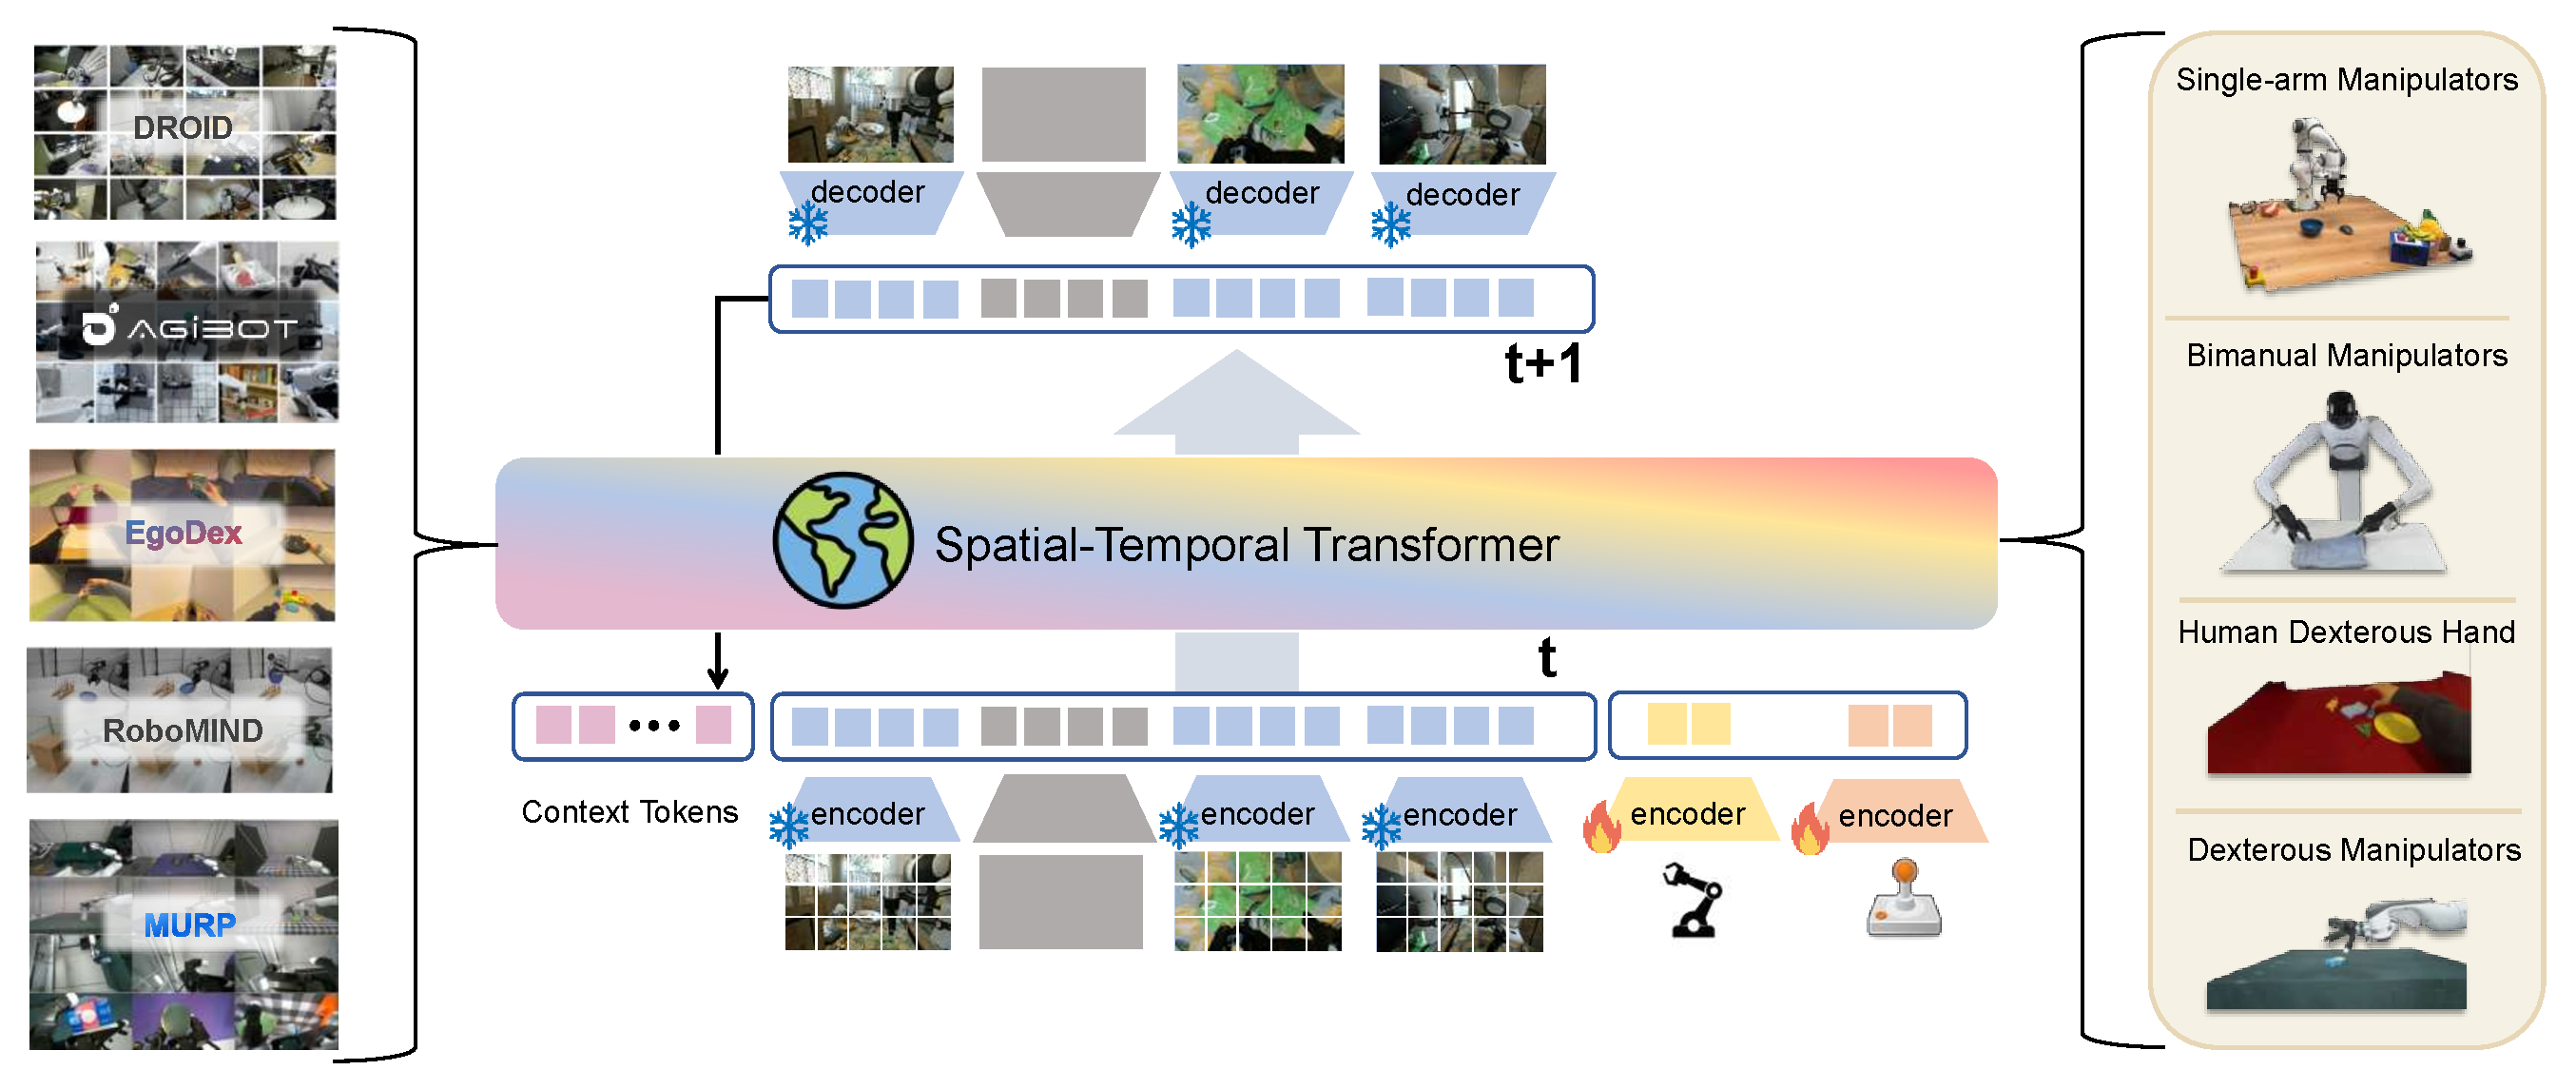
\includegraphics[width=0.9\textwidth]{figures/HWM_new.pdf}
    \caption{\textbf{Heterogeneous action-conditioned world model.}
    The world model is trained on diverse robot and human interaction datasets spanning multiple embodiments.}
    \label{fig:HWM}
\end{figure*}





\subsection{World Model Training}

The world model is a central component of \coolname{}. To support zero-shot deployment-time steering, it must be generalizable, efficient, and robust. The world model, shown in Fig.~\ref{fig:HWM}, is an action-conditioned latent dynamics model trained on heterogeneous robot and human interaction data. Its design follows three principles: multi-embodiment training for broad generalization, latent-space prediction for efficient rollout, and spatio-temporal factorization for scalable trajectory evaluation. Additional details are provided in the supplementary material.
% Section~\ref{sec:supp-world-model}.



\textbf{Multi-Embodiment Training.}
To learn a generalizable world model, we train on heterogeneous datasets~\citep{khazatsky2024droid,bu2025agibot,hoque2025egodex,wu2024robomind}, spanning single-arm manipulators, bimanual robots, dexterous hands, and human demonstrations. Visual observations are mapped into a shared latent space, while embodiment-specific action and state inputs are encoded into latent tokens using learned tokenizers. A shared spatio-temporal transformer is trained across all embodiments. The key insight is that all these embodiments interact with a shared physical world, allowing the backbone to learn transferable object interaction dynamics despite embodiment gaps. Object interaction is both the most important and most difficult component of action-conditioned prediction: robot motion is largely specified by the action input, and static scene information is already present in the observation context, while object interaction dynamics must be learned from diverse interaction data. Missing modalities are masked during training to support partially observed multi-view and multi-embodiment data.


\textbf{Latent-Space Dynamics.}
Rather than predicting pixels directly, $\mathcal{W}_\phi$ predicts future states in the latent space of a frozen DINOv2 visual encoder. DINOv2 latent representations capture rich semantic and world knowledge while preserving task-relevant structure for downstream evaluation. Pixel-space video generation is computationally expensive and often requires iterative denoising, making it poorly suited for rollout-based steering over multiple candidates. Latent-space dynamics instead enable efficient autoregressive prediction, while decoded latent rollouts can still be evaluated by an image-based value model.
In practice, latent rollout is substantially faster than video diffusion models~\cite{guo2025ctrl}: on the same NVIDIA RTX 4090 setup, generating three $320{\times}192$ frames at horizon $H{=}10$ takes 23.12\,s with a video diffusion model, compared to 0.59\,s for our latent world model.



\begin{wrapfigure}{r}{0.5\textwidth}
    \centering
    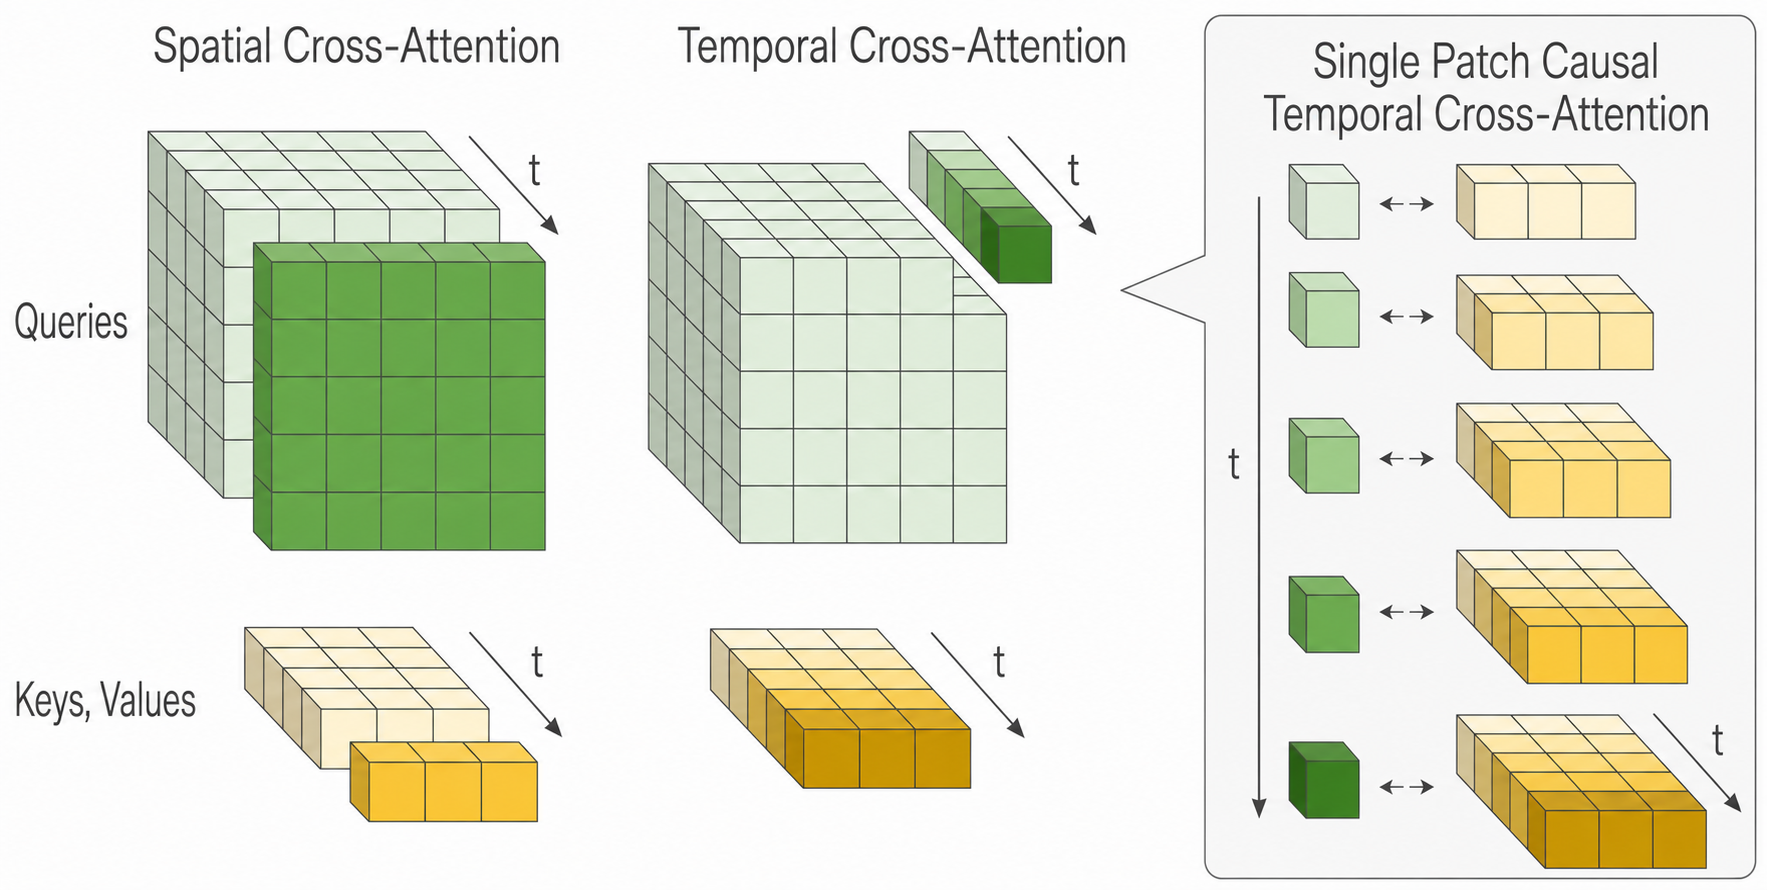
\includegraphics[width=\linewidth]{figures/cross-attention-edit.png}
    \caption{\textbf{Spatio-temporal cross attention.}
    Spatial cross-attention attends within each timestep, while temporal cross-attention applies causal attention across timesteps for each patch.
    }
    \label{fig:st-attention}
\end{wrapfigure}


\textbf{Spatio-Temporal Factorization.}
To support fast rollout over multiple candidate action chunks, we use a factorized spatio-temporal transformer~\citep{xu2020spatial}. The model consists of $N$ spatio-temporal blocks operating on visual latent tokens and action/state tokens. Each block applies self-attention to visual and control tokens together with cross-attention for action-conditioned prediction. As illustrated in Fig.~\ref{fig:st-attention}, attention is factorized into spatial attention within each timestep and causal temporal attention across timesteps for each patch. This factorization reduces attention complexity in the rollout horizon $H$ from quadratic to linear, enabling efficient evaluation of many candidate action chunks during deployment.



\subsection{\coolname{}}

\coolname{}, shown in Fig.~\ref{fig:dreamsteer}, steers a pretrained VLA policy by ranking imagined outcomes of candidate action chunks before execution. At time $t$, \coolname{} constructs a finite candidate set
\[
\mathcal{C}_t = \mathcal{C}^{\mathrm{VLA}}_t \cup \mathcal{C}^{\mathrm{prim}},
\]
where $\mathcal{C}^{\mathrm{VLA}}_t$ contains stochastic samples from the VLA policy and $\mathcal{C}^{\mathrm{prim}}$ contains predefined Cartesian action primitives. Each candidate action chunk is rolled out through the world model, decoded into image observations, and scored by the value model under instruction $\ell$. DreamSteer then executes the candidate with the highest predicted value score:
\begin{equation}
\begin{aligned}
k^\star
&=
\text{argmax}_{k \in \{1,\dots,|\mathcal{C}_t|\}}
V_\psi\!\left(
    o_t,
    \mathcal{W}_\phi(o_t,a^{(k)}_{t:t+H-1}),
    \ell
\right), 
&a^\star_{t:t+H-1}
= a^{(k^\star)}_{t:t+H-1}.
\end{aligned}
\end{equation}
Here, $\pi_\theta$, $\mathcal{W}_\phi$, and $V_\psi$ denote the policy, world model, and value model, respectively, and all remain fixed during deployment.
% Algorithm~\ref{alg:tts} summarizes the procedure.





% \begin{algorithm}[t]
% \caption{DreamSteer at Deployment Time}
% \label{alg:tts}
% \KwIn{Fixed VLA policy $\pi_\theta$, world model $\mathcal{W}_\phi$, value model $V_\psi$; instruction $\ell$; primitive action chunks $\mathcal{C}^{\mathrm{prim}}$; number of VLA proposals $K_{\mathrm{VLA}}$; horizon $H$.}
% \KwOut{Action chunks executed on the robot.}

% \While{task not complete}{
%     \textbf{Observe:} receive the current observation $o_t$\;

%     \textbf{Propose:} sample $K_{\mathrm{VLA}}$ action chunks from the VLA policy $\pi_\theta(\cdot \mid o_t, \ell)$ and store them in $\mathcal{C}^{\mathrm{VLA}}_t$\;

%     \textbf{Augment:} combine VLA samples with primitive chunks,
%     $\mathcal{C}_t \leftarrow \mathcal{C}^{\mathrm{VLA}}_t \cup \mathcal{C}^{\mathrm{prim}}$\;

%     \For{each candidate action chunk $a^{(k)}_{t:t+H-1} \in \mathcal{C}_t$}{
%         \textbf{Imagine:} predict its future observations,
%         $\hat{o}^{(k)}_{t+1:t+H} \leftarrow
%         \mathcal{W}_\phi(o_t, a^{(k)}_{t:t+H-1})$\;

%         \textbf{Score:} evaluate the imagined rollout,
%         $S^{(k)} \leftarrow
%         V_\psi(o_t, \hat{o}^{(k)}_{t+1:t+H}, \ell)$\;
%     }

%     \textbf{Select:} choose the highest-scoring candidate,
%     $k^\star \leftarrow \arg\max_k S^{(k)}$\;

%     \textbf{Execute:} run the selected action chunk
%     $a^{(k^\star)}_{t:t+H-1}$ on the robot\;

%     \textbf{Replan:} observe the next decision point and repeat\;
% }
% \end{algorithm}




\paragraph{Stochastic Policy Action Proposals.}
The policy $\pi_\theta$ is instantiated as a pretrained VLA model. We write the per-step observation as
\[
o_t =
\{
I_t^{\mathrm{wrist}},
I_t^{\mathrm{ext}},
s_t^{\mathrm{robot}},
s_t^{\mathrm{gripper}}
\},
\]
where $I$ denotes visual observations and $s$ denotes proprioceptive state. Conditioned on $o_t$ and $\ell$, the policy samples $K_{\mathrm{VLA}}$ temporally extended action chunks:
\[
a^{(k)}_{t:t+H-1}
\sim
\pi_\theta(\cdot \mid o_t,\ell),
\qquad
k=1,\dots,K_{\mathrm{VLA}}.
\]
These samples expose diverse behaviors already present in the generative action distribution of the pretrained policy.

We augment these policy samples with a small primitive library $\mathcal{C}^{\mathrm{prim}}$. The primitive library consists of fixed short-horizon Cartesian motions, including end-effector translations along left/right, up/down, and forward/backward directions, as well as gripper open and close commands. Each primitive is represented as an action chunk of length $H$, making it temporally aligned with VLA-generated chunks. The primitives are not intended to solve manipulation tasks on their own. Instead, they provide simple alternatives that improve candidate coverage when the VLA samples alone fail to make progress, for example when the end effector is near the target object but the sampled actions do not move into a grasp-ready pose.

\paragraph{World Model Predictive Visual Dynamics.}
The world model $\mathcal{W}_\phi$ predicts future observations conditioned on the current observation and a candidate action chunk:
\[
\hat{o}^{(k)}_{t+1:t+H}
=
\mathcal{W}_\phi(o_t,a^{(k)}_{t:t+H-1}).
\]
Internally, the model operates in the latent space of a frozen DINOv2 visual encoder \citep{oquab2023dinov2}. Suppressing modality-specific tokenization for clarity, the rollout can be written as
\begin{equation}
z_t = E(o_t), \quad
\hat{z}^{(k)}_{t+1:t+H}
=
F_\phi\!\left(z_t,a^{(k)}_{t:t+H-1}\right), \quad
\hat{o}^{(k)}_{t+1:t+H}
=
D\!\left(\hat{z}^{(k)}_{t+1:t+H}\right).
\end{equation}
where $E$ is the frozen observation encoder, $F_\phi$ is the learned latent dynamics model, and $D$ is the frozen decoder that reconstructs visual observations from predicted latents. 

\paragraph{Value Function Scoring and Steering Decision.}
The value function $V_\psi$ is instantiated as a pretrained Vision-Language-Action-Critic (VLAC) model \citep{zhai2025vision} based on the InternVL2-2B architecture \citep{chen2024expanding}. VLAC provides an instruction-conditioned progress signal over pairs of visual observations. Given an imagined rollout for candidate $k$, we compute a trajectory-level score by summing pairwise progress estimates along the decoded rollout:
\begin{equation}
S^{(k)}
=
\sum_{j=1}^{H}
\mathrm{VLAC}
\!\left(
    \hat{o}^{(k)}_{t+j-1},
    \hat{o}^{(k)}_{t+j},
    \ell
\right),
\qquad
\hat{o}^{(k)}_{t} = o_t .
\end{equation}
This score estimates how much the candidate action chunk advances the task specified by $\ell$. DreamSteer does not require the value model to produce calibrated absolute rewards; it only needs the scores to rank candidates generated at the same timestep. The system then executes the action chunk with the highest score, steering the pretrained VLA policy toward predicted outcomes that better satisfy the language instruction.


